%% SIGCHI Proceedings Format (modern) Sample Document
%% This sample file demonstrates the use of the `sigchi-modern' class file.
%%
%% The content of this document draws heavily on the `HCI Archive Format'
%% template supplied by SIGCHI, but has been modified to demonstrate and
%% document the LaTeX class.

% The parameter given to the `\documentclass' command can be one of:
%   `preprint', `submission', or `final'.
% These control the presence of certain features for each stage of the authoring
% process. For example, `submission' does not output the author block, and
% `final' disables page numbers.
%
% The \preprintonly{}, \submissiononly{}, and \finalonly{} commands allow you
% to wrap text that will only be output under the corresponding option.
\documentclass[preprint]{sigchi-modern}

\def\meta/{\preprintonly{\textsc{MeTA}}\finalonly{\textsc{MeTA}}%
\submissiononly{(redacted)}}

\newcommand{\citemeta}{\preprintonly{\cite{Massung:2016:ACL}}%
  \finalonly{\cite{Massung:2016:ACL}}%
  \submissiononly{[redacted citation]}}

% These packages aren't required, but do provide some helpful features that are
% used in this sample.
\usepackage{graphicx}  % Graphics for figures
\usepackage{booktabs}  % Nice formatting for tables
\usepackage{balance}   % Attempts to balance the columns on the last page

% A nice way to help avoid overful lines handing out into the margins is the
% `microtype' package, which lets certain characters extrude a *little* bit.
\usepackage{microtype}
% If the situation becomes dire, use:
%\sloppy

% You may use any bibliography package as long as the output matches that of
% the prescribed format. `natbib' is a fairly nice default, and the provided
% BibTeX style file has been tested with it.
\usepackage[numbers]{natbib}
\bibliographystyle{acm-sigchi-modern}

% Define these tokens as appropriate for the conference to generate the
% necessary copyright notice for `final` mode.
\confname{CHI'14}
\confdate{April 26--May 1}
\confyear{2014}
\conflocation{Toronto, Canada}
\procissn{XXX-X-XXXX-XXXX-X/XX/XX}
\doi{10.1000/182}
% \copylicense be set to one of: \acmcopyright, \authorlicense, or \openlicense
\copylicense{\authorlicense}

% End of preamble. Here comes the document.
\begin{document}

\title{Modeling MOOC Student Behavior With Two-Layer Hidden Markov Models}

% Author information can be set automatically if you provide a series of
% author names and affiliations:
%   \author[1]{Author One}
%   \author[2]{Author Two}
%   \author[1,2]{Author Three}
%   \affiliation[1]{Organisation One\\
%                   Some Country}
%   \affiliation[2]{Organisation Two\\
%                   Some Country}
%   \authorextra{\mailto{one@example.com}, \mailto{two@example.org},
%                \mailto{three@example.net}}
% Or, manually:
%   \author{
%     \authorname{Author One}\\
%     \authoraffil{
%       Organisation One\\
%       Some Country\\
%       \mailto{one@example.com}}}
%   \author{
%     \authorname{Author Two}\\
%     \authoraffil{
%       Organisation Two\\
%       Some Country\\
%       \mailto{two@example.org}}}
% Refer to the body text of the document for more details.
\author[1]{Chase Geigle}
\author[1]{ChengXiang Zhai}

% Set \authorwidth with the longest author name if you don't like the default
% spacing:
\settowidth{\authorwidth}{ChengXiang Zhai1}
\settowidth{\affilwidth}{University of Illinois at Urbana-ChampaignAAA}

\affiliation[1]{Department of Computer Science\\
    University of Illinois at Urbana-Champaign\\
    Urbana, Illinois, USA}

\authorpostscript{\email{\{%
  \href{mailto:geigle1@illinois.edu}{geigle1},
  \href{mailto:czhai@illinois.edu}{czhai}\}@illinois.edu}}

% If you format the author blocks manually, use \authorlist with a
% comma-delimited list of the author names.
% This is written into the PDF metadata for preprint and final modes.
%\authorlist{Author One, Author Two, Author Three, Author Four}

% Produces the title, author, and optional banner block.
\maketitle

\begin{abstract}
  Massive open online courses (MOOCs) provide educators with an abundance
  of data describing how students interact with the platform, but this data
  is highly underutilized today. This is in part due to the lack of
  sophisticated tools to provide interpretable and actionable summaries of
  huge amounts of MOOC activity present in log data. In this paper, we
  propose a method for automatically discovering student behavior patterns
  by leveraging the click log data that can be obtained from the MOOC
  platform itself in a completely unsupervised manner.
\end{abstract}

% A semicolon-separated list of keywords to describe the paper.
\keywords{MOOC log analysis; student behavior modeling; Markov models;
hidden Markov models}

\newcommand{\NSFGRFP}{This material is based upon work supported by the
National Science Foundation Graduate Research Fellowship Program under
Grant Number DGE-1144245.}

\newcommand{\acknowledgments}{The authors would like to thank Hao Zheng,
Jason Cho and Sean Massung for their helpful discussion while developing
this work, and the ATLAS group at UIUC for their help with securing the
datasets used. \NSFGRFP{}}

% ACM classification block.
% \category{}{}{}[] has three mandatory arguments and one optional argument; it
% can be used multiple times.
%\classification{%
%    \category{}{}{}
%}

\section{Introduction}
The proliferation of massive open online courses (MOOCs) has resulted in a
profound impact on education. As more and more learners turn to MOOCs to
educate themselves on various topics, more and more behavioral data is
being collected as part of the system on which the MOOC is offered. The
data present in these logs has the power to aid us in understanding the
behavior of students who take our MOOCs, which is mostly undetectable for
instructors of these MOOCs today due to its vast scale. As a result, the
rich data available through these MOOC logs is highly underutilized today.

What stands in the way? Clearly, intelligent systems to create concise and
digestible summaries of the massive amount of interaction data collected
are needed in order to empower the instructors of these courses. If we can
understand how users are interacting with our MOOCs, we are much more
likely to be able to make changes to these courses that positively impact
learners. While we can easily observe the changes in behavior of students
in real classrooms, MOOCs present a challenge due to their hands-off
nature and sometimes irregular schedule due to being a full-time worker.   
We view this paper as attempting to bridge this gap. Specifically,
in this paper we propose unsupervised learning methods for automatically
discovering and characterizing student learning behavior patterns or profiles from large
collections of click logs associated with MOOCs. 

Our work is motivated by the following observations:
\begin{enumerate}
  \item Student behavior is complicated and cannot necessarily be captured
      sufficiently by rule-based methods such as those explored by
      \citet{Kizilcec:2013:LAK} and \citet{Davis:2016:EDM}. We instead
      propose to treat student behavior patterns as being characterized
      (represented) via a sequence of \emph{latent states}. This allows us
      to automatically capture patterns that we might not have been able to
      articulate clearly a priori via a series of rules, and also allows us
      to model the inherent uncertainty in assigning a student's behavior
      to a particular pattern or group.
  \item Student behavior can vary over time. Previous models that treat students
      as exhibiting only one behavioral pattern over
      time~\cite{Faucon:2016:EDM} miss out on the opportunity to understand
      student behavior dynamics in a course. We propose a latent space
      model with {\em latent state transitions} to flexibly model the
      dynamics.
  \item Analysis of student behavior can and should be performed at varying
      levels of granularity. This requires us to aggregate data over time
      with \emph{different levels of resolution}; existing models tend to come
      with a particular assumption about the resolution of time they
      consider~\cite{Faucon:2016:EDM, Kizilcec:2013:LAK, Shih:2010:EDM}. We
      propose a more flexible model to accommodate different levels of
      resolution.
\end{enumerate}

Thus, what we propose is a \emph{latent variable approach} to mining student behavior
patterns that is \emph{probabilistic} for inference and 
\emph{flexible to model state changes over different time resolutions}. 
More specifically, we propose a novel two-layer hidden Markov model (2L-HMM) to
 discover latent student behavior patterns via
unsupervised learning on large collections of student behavior observation
sequences. Evaluation results on a MOOC data set on Coursera demonstrate that 2L-HMM can effectively 
discover a variety of interesting interpretable student behavior patterns at different levels of resolution, many of which are beyond what existing approaches can discover. 2L-HMM further enables easy use of the discovered patterns for discriminative analysis such as prediction of learning outcome. 
Since our proposed methods are unsupervised, they can potentially be applied to any MOOC data without requiring any manual work to facilitate understanding of student behaviors and their variations, opening up many possibilities for developing intelligent tutoring systems that can adaptive to student behavior. 




\section{Related Work}

Our model is based heavily upon the prior art of Hidden Markov
Models~\cite{Rabiner:1990:RSR} for sequence labeling tasks. These types of
models are widely applicable and have been used for tasks such as speech
recognition~\cite{Huang:1990:HMM}, part-of-speech
tagging~\cite{Jurafsky:2009:SLP}, and econometrics~\cite{Hamilton:1990:JoE}
and are a member of the more general family of probabilistic graphical
models~\cite{Koller:2009:PGM}.  A major challenge in applying HMMs and
other graphical models successfully to solve a problem is to design an
appropriate architecture of the model, which always varies according to
specific applications.

For example, in part-of-speech tagging~\cite{Jurafsky:2009:SLP} the output
distributions are categorical (distributions over words from a fixed
vocabulary) and the latent states represent the part-of-speech category for
a word. In speech recognition~\cite{Huang:1990:HMM} the output
distributions might be mixtures of Gaussians to predict real-valued vectors
extracted from short windows of a speech signal. In the domain of
econometrics, \citet{Hamilton:1990:JoE} explores HMMs in the context of
``regime-switching.'' In this framing, the goal is to understand how
econometric data changes by modeling discrete changes in ``regime'' as
having an impact on the resulting real-valued vector data observed. The
``regimes'' are represented with some sort of model that can produce
real-valued vector data, such as a multivariate Gaussian or an
auto-regressive model. The analogy with HMMs is that a ``regime'' is a
latent state, and the characterization of the regime itself is the output
distribution for that latent state. Our model can be seen as such a
``regime-switching'' model where the output of the ``regimes'' that
students are switching between are discrete-valued \emph{sequences} (as
opposed to real numbers, vectors of real numbers, or categorical symbols)
and the model used to represent a specific ``regime'' is an (observable)
Markov chain over the observed student actions. We view the switching
between ``regimes'' as the first ``layer'' of our model, and the
transitioning behavior \emph{within} a ``regime'' between the actions a
student takes as the second ``layer'' of our model.

A multi-layered approach to HMM modeling of sequence data has been
performed before in other domains. \citet{Zhang:2004:CVPR}, for example,
explored a two-layer HMM framework for modeling actions in meetings, but
their definition of ``two-layer'' differs from ours. In their formulation,
the ``lower-layer'' level is used to label audio-video action sequences
into basic events, and the ``upper-layer'' is used to label the output of
the lower-layer to discover higher-level office behavior abstractions. Our
formulation differs in that we do not feed the labeled sequence of the
lower level into the input of the higher level. Instead, our lower level is
actually treated using a non-hidden Markov model, and the higher level is
modeling transitions between the $K$ different non-hidden Markov models we
consider.

Our formulation is more closely related to the Hierarchical Hidden Markov
Model (HHMM) detailed in \citet{Fine:1998:ML}. Here, the ``layers'' are
modeled by having the hidden Markov model have two kinds of transitions.
Horizontal transitions move between states within a layer, where vertical
transitions move between different layers. At the bottom layer lie the
``production'' states, which output symbols according to some probability
distribution. Our specific model in this case can be modeled as a HHMM
where the horizontal transitions between nodes at the highest layer
(including self-loops) \emph{must} be immediately followed by a vertical
transition to the lower layer. The output probability distributions over
symbols in the lower layer ``production'' level are forced to emit only one
kind of symbol, and vertical transitions are only allowed into the original
higher-layer state that transitioned down into the lower-layer.

Mixtures of hidden Markov models are also conceptually similar to our
formulation. \citet{Song:2009:NDSS} explored using a mixture of hidden
Markov models in the context of anomaly detection in the security domain.
\citet{Ypma:2002:Springer} use mixtures of HMMs to categorize web pages and
cluster users by investigating web log data, which is quite similar to the
clickstream log data we obtain from MOOCs. The major difference between
our approach and a standard mixture of HMMs is that we also model the
\emph{transition behavior} between the Markov models that make up our
model's lowest layer, where a standard mixture of HMMs would ignore the
potential dependence of the previous sequence's latent state on the next
sequence's latent state.

HMMs or similar ideas have been previously applied to model education
data~\cite{Shih:2010:EDM,Kizilcec:2013:LAK,Davis:2016:EDM}, but the
previous models are not well tuned toward the student behavior task and
thus cannot adequately address all the aspects of complexity of student
learning behavior.  A main technical contribution of this paper is to
propose a more general HMM that can better adapt to the variations of
student behavior via its variable resolution and nested HMM structure, and
thus enable discovery of more sophisticated behavior patterns and provide
more detailed characterization of student behavior than the previous
models.

For example, \citet{Kizilcec:2013:LAK} assigned students to states
following a rule-based approach based upon when the student submitted the
assignment for a particular week in the course. They investigated how
students transitioned between these states as the course progressed, and
used the sequence of states a student exhibited as a representation for
performing $k$-means clustering of students into related groups. This
differs from our method substantially: we assign students to states using a
probabilistic framework to account for uncertainty in this state
assignment, and jointly learn \emph{representations} for these states,
which are treated as being \emph{latent} as opposed to pre-defined using
some rule (or set of rules).  Furthermore, our model provides more
flexibility in how the time segments are defined, allowing for both finer
(for example, day-by-day) or coarser (for example, month-by-month)
granularity. \citet{Shih:2010:EDM} investigated the use of HMM-based
clustering techniques for automatic discovery of student learning
strategies when solving a particular problem.  This is similar to our
approach in that the description of behavior profiles is a Markov model,
but cannot further characterize each latent state with another informative
HMM. Thus their work can be regarded to modeling ``micro'' behavior,
whereas our model can model both ``micro'' and ``macro'' behavior.

\citet{Davis:2016:EDM} investigate frequent student behavior pattern chains
with a set of actions that is defined similarly to ours. However, their
method for finding the common behavioral patterns involves a manual
clustering step to identify behavioral ``motifs,'' which is then followed
by an automatic (rule-based) assignment of all sequences to these motifs.
Our method, by contrast, attempts to do this automatically: the latent
state representations obtained by our model attempt to capture similar
meanings to their behavior motifs in a completely automated fashion. They
also automatically generate and investigate Markov models for different
MOOCs, but do so by considering \emph{all} student action sequences as
belonging to a \emph{single Markov model}. In our approach, we allow each
student behavior sequence to belong to one of $K$ different Markov models
(and further model the transition probabilities between these latent state
Markov models between each sequence a student generates). Thus, their
Markov models presented are a special case of our model when $K = 1$.

\citet{Faucon:2016:EDM} proposed a semi-Markov model for simulating MOOC
students. They produce behavior profiles that characterize groups of
students in the form of semi-Markov models like our proposed model does,
but they assume that a student can belong to only one behavior profile
across the entire course rather than allowing this profile to change over
time. Because we do not have this restriction, our model is also able to
learn the transition probabilities between the different behavior profiles
we discover.

There are a few additional related studies worth mentioning.
Bayesian Knowledge Tracing~\cite{Corbett:1994:UMUAI} in its basic form uses
a hidden Markov model to model the probability that a learner knows a
certain skill at a given time. Modifications to this algorithm include
contextual estimation of the ``slip'' and ``guess'' probabilities of the
model~\cite{Baker:2008:ITS} and most recently a re-framing as a neural
network problem~\cite{Piech:2015:NIPS}.



\section{A Two-Layer HMM for MOOC Log Analysis}

\subsection{Basic idea and rationale} 

Our general idea is to use a probabilistic generative model to model 
the student activities as recorded in a MOOC log, which means we will 
assume that all the observed student activities are samples drawn (i.e., ``generated'') from 
a parameterized probabilistic model. We can then estimate the 
parameter values of the probabilistic model by fitting the model to a specific
MOOC log data set. The estimated parameter values could then be treated as 
the latent ``knowledge'' discovered from the data. Because such a generative model 
attempts to fit {\em all} the data, it enables us to discover interesting patterns
that can explain the {\em overall} behavior of a student or the {\em common} behavior patterns shared by many students. 

HMM is a specific probabilistic generative model with a ``built-in'' state transition system
that would control the data to be generated by the model, thus it is especially 
suitable for modeling sequence data. At any moment, the HMM would be in 
one of $k$ states $U=\{u_1, ...,u_k\}$, and at the next moment, the HMM would move to 
another state stochastically according to a transition matrix that specifies the probability of
going to state $u_i$ when the HMM is currently in state $u_j$, i.e., $p(u_i|u_j)$. 
When the HMM is in state $u$, the HMM can generate an observable data point $x$ 
according to an output probabilistic model $p(x|u)$. Thus if we ``run'' an HMM for 
$N$ time points denoted by $t=1, ..., N$, the HMM could ``generate'' a sequence of 
observations $x_1 ... x_N$, where each $x_i$ is an output symbol by 
going through a sequence of {\em hidden states} $w_1 ... w_N$ where $w_i \in U$ is a state. 
The association of such a latent sequence of state transitions with the observed symbols makes
it possible to use HMM to ``decode'' the latent behavior of students behind the surface behavior we directly observe in the log data, allowing for understanding student behavior more deeply than a model with no latent state variables. 

In many ways, the generation process behind an HMM is meant to simulate the actual behavior of a student in the following sense: First, students may be in different ``task state'' (or ``behavior state'')  in the process of study. 
For example, one task state may be to learn about a topic by mostly watching lecture videos, another task state may be to work on quizzes, and yet another may be to participate in forum discussions. While in each of these different states, the student would tend to exhibit different surface ``micro'' behaviors. For example, in the lecture study state, the student would tend to have many video-watching related behaviors and occasionally forum activities, while in the quiz-taking state (in order to pass each module), the student would tend to show many quiz-related ``micro'' activities as well as asking questions or checking disussions on the forum. Note that due to the complexity of the student behavior, it is very difficult to accurately {\em prescribe} the specific surface ``micro'' behavior patterns for each state, especially without  prior knowledge about the students. For example, forum activities are likely interleaved with other activities   in every task state and the interleaving pattern can be somewhat irregular with potentially many variations. 
A major motivation for using an HMM is because 1) it uses a probabilistic model (i.e., the output probability distribution $p(x|u)$ conditioned on each state) to directly capture the inevitable uncertainty in the association of surface ``micro'' activities with their corresponding latent task/behavior state, which is often our main taraget to discover and characterize, and 2) it does not make any assumption about which latent task/behavior state must be associated with which observed activities or how a student would move from one state to another, but instead let our data ``tell'' us what kind of associations are most likely and what kind of transitions are most often, and which states tend to be more long-lasting for any particular set of students. 

However, if we are to use an ordinary HMM to analyze our data, we would treat each observed ``micro'' activity (e.g., video watching, or forum post reading) as an output symbol, and thus the output distribution $p(x|u)$ for each discovered latent state would be a simple distribution over all kinds of observable micro activities recorded in our log data (e.g., 50\% lecture watching, 8\% quiz taking, 7\% quiz submission, 2\% course wiki reading, ...). While such a distribution is meaningful and can already help us intepret the corresponding latent state, it only gives us a rather superficial characterization of student behavior. Ideally, we want $p(x|u)$ to characterize the directly observable behavior in more detail to further capture the relations and dependencies of these micro activities. To this end, we would treat an {\em entire sequence} of micro activities (e.g., one session of activities) as an observed ``symbol'' from a latent state, and further model the generation of such a sequence with another Markov model where we treat each micro activity as an {\em observable} state, and model the transitions between these activity states in very much the same way as the state transitions in HMM.  Combining this ``surface'' Markov model with the ``deep'' hidden Markov model gives us a fairly general and powerful two-layer HMM (TL-HMM) that can simultaneously learn ``deeply'' the latent task/behavior states and their transitions as well as the corresponding ``surface'' activity transition patterns associated with each latent state to facilitate interpretation and analysis of the discoverd latent state patterns. Next, we present this model more formally and discuss how to estimate its parameters. 

\subsection{Formal definition of TL-HMM}

Given a MOOC log, we can define a set $\mathbf{A}$ of actions that a
student can take at any given time. For example, an action $a \in
\mathbf{A}$ might be ``viewing lecture'', ``taking quiz'', or ``viewing
forum''. For each student in the course $\ell \in \mathbf{L}$, we then
extract a list of action sequences $\mathbf{S}_\ell$ that he or she
produced as observed in the log, where each sequence $\mathbf{s} \in
\mathbf{S}_\ell$ is itself a list of actions $(a_1, a_2, \ldots, a_M)$ with
each $a_i \in \mathbf{A}$.  Each sequence can be divided flexibly; in this
paper we chose to denote the end of a sequence as occurring when no further
actions occur within a 10 hour window of time (and thus our sequences
roughly correspond to one day's worth of activity).

Each sequence $\mathbf{s} \in \mathbf{S}_\ell$ is associated with a latent
state $u \in \{1,\ldots,K\}$ (where $K$ is a fixed constant picked in
advance). The actions within the sequence $\mathbf{s} = (a_1, a_2, \ldots,
a_M)$ are then modeled as a first-order Markov process conditioned upon $u$
where each action is drawn from a distribution conditioned upon the
previous action (except for the first which is sampled from an initial
starting distribution). We can write the parameters for the first-order
Markov model associated with latent state $u$ as $\lambda^{(u)} =
(\pi^{(u)}, A^{(u)})$ where $\pi^{(u)}$ indicates the initial probability
vector of length $|\mathbf{A}|$ and $A^{(u)}$ is an $|\mathbf{A}| \times
|\mathbf{A}|$ matrix indicating the transition probabilities between each
pair of actions from $\mathbf{A}$.

Thus, the probability of a sequence $\mathbf{s}$ of length $M$ given its
latent state $u$ is
\begin{equation}
  P(\mathbf{s} \mid \lambda^{(u)}) = P(a_1 \mid \pi^{(u)}) \prod_{i=2}^M P(a_i \mid
  a_{i-1}, A^{(u)})
\end{equation}
where $P(a \mid \pi^{(u)}) = \pi^{(u)}_a$ is the probability of starting
with action $a$ and $P(a_i \mid a_{i-1}, A^{(u)}) = A^{(u)}_{a_{i-1}, a_i}$
is the transition probability of moving from action $a_{i-1}$ to $a_{i}$.

We can compute the likelihood of a list of action sequences
$\mathbf{S}_\ell$ of length $N$ for a student $\ell$ as
\begin{equation}
  P(\mathbf{S}_\ell \mid \Lambda)
  = \prod_{i=1}^N \sum_U P(U \mid \Lambda) P(\mathbf{s}_i \mid
  \lambda^{(u_i)})
\end{equation}
where $\Lambda$ is the set of all model parameters, and the summation over
$U$ indicates a sum over all possible latent state sequences of length
$|\mathbf{s}_i|$. In our model, we let $\Lambda = (\pi, A, \lambda^{(1)},
\ldots, \lambda^{(K)})$ where $\pi$ and $A$ are the parameters of a first-order
Markov model over the latent states and each $\lambda^{(i)}$ consists of
the parameters for the first-order Markov model over action sequences for
latent state $i$. Thus $\pi$ (without superscripts) is an initial
probability vector of length $K$ and $A$ (without superscripts) is a $K
\times K$ transition probability matrix, analogous to the case with the
individual first-order Markov model parameters $\lambda^{(i)}$ for each
latent state.

This can be seen as a modification of the traditional hidden Markov
model~\cite{Rabiner:1990:RSR} where instead of discrete observations (one
for each latent state transition) we have observations that take the form
of entire sequences $\mathbf{s}_i = (a_1, a_2, \ldots a_M)$ whose
probabilities are computed using another (non-hidden) Markov model
conditioned upon the latent state $u_i$.

\subsection{Parameter Estimation}
To learn the parameters of our model, we may attempt to use maximum
likelihood estimation. Unfortunately, a closed-form solution does not
exist, so we must appeal to the EM algorithm~\cite{Dempster:1977:JRSS}. In
particular, we propose a minor modification of the Baum-Welch
algorithm~\cite{Rabiner:1990:RSR} which is used to learn the parameters for
hidden Markov models. In the following sections, we will provide a brief
description of the original Baum-Welch algorithm, and then describe our
modification.

\subsubsection{Baum-Welch for Traditional HMMs}
In the traditional HMM formulation, we have $\Lambda = (\pi, A, B)$ where
$\pi$ is the initial probability distribution over the latent states,
$A$ is a $N\times N$ matrix indicating the latent state transition
probabilities, and $B$ is a $N \times V$ matrix indicating the probability
of generating a discrete observation symbol from a given latent state. The
Baum-Welch algorithm (also called the forward-backward algorithm) defines
two sets of variables $\alpha_t(i)$ called the forward variables and
$\beta_t(i)$ called the backward variables.

$\alpha_t(i) = P(o_1, \ldots, o_t, q_t = i \mid \Lambda)$ is the probability of
generating the sequence of observations $(o_1, o_2, \ldots, o_t)$ up to time
$t$ and arriving in state $i$ at that time. They are typically defined
using the following recursion:
\begin{itemize}
  \item $\alpha_1(i) = \pi_i b_i(o_1)$, the probability of starting in
    state $i$ ($\pi_i$) times the probability of generating the first
    observation $o_1$ from state $i$.
  \item $\alpha_{t+1}(i) = b_i(o_{t+1})\sum_{j=1}^N \alpha_t(j) A_{ji}$,
    the probability of generating the observation $o_{t+1}$ from state $i$
    times the probability that we arrive in state $i$ from any other
    previous state after generating all of the other observations.
\end{itemize}

Analogously, $\beta_t(i) = P(o_{t+1}, \ldots, o_{T} \mid q_t = i, \Lambda)$
is the probability of generating the \emph{rest of the sequence} given that
we are in state $i$ at time $t$. They are also defined using a recursion:
\begin{itemize}
  \item $\beta_T(i) = 1$
  \item $\beta_t(i) = \sum_{j=1}^N \beta_{t+1}(j) A_{ij} b_j(o_{t+1})$, the
    probability of transitioning to any state $j$ and generating the
    observation $o_{t+1}$ times the probability of generating the rest of
    the sequence given that we transitioned to state $j$.
\end{itemize}

Given the $\alpha$s and the $\beta$s, we can compute $\gamma_t(i)$, the posterior
probability of being in a given state $i$ at time $t$, and $\xi_t(i,j)$,
the posterior probability of going through a transition from state $i$ to
state $j$ at time $t$ as
\begin{equation}
  \gamma_t(i) = \frac{\alpha_t(i)\beta_t(i)}{\sum_{j=1}^N
  \alpha_t(j)\beta_t(j)}
\end{equation}
and
\begin{equation}
  \xi_t(i,j) = \frac{\alpha_t(i) A_{ij} b_j(o_{t+1}) \beta_{t+1}(j)}
  {\sum_{j=1}^N \alpha_t(j)\beta_t(j)}
\end{equation}
respectively. This is the E-step of the EM algorithm.

Given $\gamma_t(i)$ and $\xi_t(i,j)$ for each sequence $\mathbf{o}_k$ in
some training data of length $M$, we can update our model parameters
$\Lambda$ as
\begin{align}
  \pi_i &= \frac{\sum_{k=1}^M \gamma^{(\mathbf{o}_k)}_1(i)}{M},\\
  A_{ij} &= \frac{\sum_{k=1}^M \sum_{t=1}^T \xi^{(\mathbf{o}_k)}_t(i,j)}
  {\sum_{k=1}^M \sum_{j=1}^N \sum_{t=1}^T \xi^{(\mathbf{o}_k)}_t(i,j)},
  \text{ and }\\
  b_i(v) &= \frac{\sum_{k=1}^M \sum_{t=1, o_{k,t} = v}^T
  \gamma^{(\mathbf{o}_k)}_t(i)}
  {\sum_{k=1}^M \sum_{t=1}^T \gamma^{(\mathbf{o}_{k,t})}_t(i)}.
\end{align}
This is the M-step of the EM algorithm.

\subsubsection{Baum-Welch for HMMs with Sequence Observations}
The major deviation of our model from the traditional HMM is that our
observations are themselves sequences. Thus, in all of the equations
presented in the previous section, we treat an observation $o_t =
\mathbf{s}_t$ at time $t$ as consisting itself of a list of actions $(a_1,
\ldots, a_M)$. Thus, instead of defining $b_i(v)$ as the probability that a
discrete observation \emph{token} $v$ is generated from state $i$, we have
\begin{equation}
  b_i(\mathbf{s}_t) = P(\mathbf{s}_t \mid \lambda^{(i)})
  = P(a_1 \mid \pi^{(i)}) \prod_{k=2}^M P(a_k \mid
  a_{k-1}, A^{(i)})
\end{equation}
where $b_i(\mathbf{s})$ now defines the probability of an action sequence
using a first-order (non-hidden) Markov model.

Fortunately, the recursions for the $\alpha$ and $\beta$ variables remain
the same, as do the definitions of $\gamma_t(i)$ and $\xi_t(i,j)$ in the
E-step. The only change is in the updating equations in the M-step,
where we replace the update for $b_i(v)$ by a pair of updates: one for
$\pi^{(i)}_a$ one for $A^{(i)}_{ab}$. We denote the $m$-th action in the
$t$-th sequence for the $k$-th student as $o_{k,t,m}$. The two updates can
be written as
\begin{align}
  \pi^{(i)}_{a}
  &= \frac{\sum_{k=1}^M \sum_{t=1,a_1 = a}^T \gamma^{(\mathbf{o}_k)}_t(i)}
  {\sum_{k=1}^M \sum_{t=1}^T \gamma^{(\mathbf{o}_k)}_t(i)}, \text{ and }\\
  A^{(i)}_{ab}
  &= \frac{\sum_{k=1}^M \sum_{t=1}^T
  \sum_{m=2,a_{m-1}=a \land a_m = b}^{|\mathbf{o}_{k,t}|}
  \gamma^{(\mathbf{o}_k)}_t(i)}
  {\sum_{k=1}^M \sum_{t=1}^T \sum_{m=2}^{|\mathbf{o}_{k,t}|}
  \gamma^{(\mathbf{o}_k)}_t(i)}
\end{align}
where $a_m = o_{t,k,m}$ (for notational conciseness). Our modified EM
algorithm for HMMs with sequence observations is provided as part of the
\meta/ toolkit~\citemeta{}.


\newcommand{\textretrieval}{\preprintonly{textretrieval-001}%
    \finalonly{textretrieval-001}%
    \submissiononly{moocname1-00X}}

\newcommand{\sustain}{\preprintonly{sustain-001}%
    \finalonly{sustain-001}%
    \submissiononly{moocname2-00X}}

\newcommand{\UIUC}{\preprintonly{UIUC}%
    \finalonly{UIUC}%
    \submissiononly{(redacted University)}}

\section{Results}
To qualitatively evaluate our model, we can look at the latent state
representations we learn by fitting the model to some MOOC log data. We can
also inspect the transition matrix between the latent states discovered by
the model.

Specifically, we look at the MOOC logs associated with two different
Coursera MOOCs offered by \UIUC{}: \textretrieval{} and \sustain{}.  The
\textretrieval{} MOOC represents a highly technical computer science course,
where the \sustain{} MOOC is more representative of a humanities course. We
picked these two MOOCs because of their vastly different content domains.
Table~\ref{table:datasets} summarizes the two datasets we extracted from
the MOOCs.

\begin{table}
  \begin{center}
    \begin{tabular}{rrrr}
      \textbf{MOOC} & \textbf{Students} & \textbf{Sequences} & \textbf{Avg.
      $|\mathbf{s}|$}\\\hline
      \textretrieval{} & 18,941 & 85,240 & 7.31\\
      \sustain{} & 85,240 & 231,881 & 15.4
    \end{tabular}
    \caption{Statistics about the sequences extracted from the two MOOCs.}
    \label{table:datasets}
  \end{center}
\end{table}

\subsection{Latent State Representations}
First, we fit a 6-state TL-HMM to the \textretrieval{} sequence dataset and
show some of the latent state representations we find. We used the
following ten actions as our action set $\mathbf{A}$:
\begin{enumerate*}[label=(\arabic*)]
  \item quiz start,
  \item quiz submit,
  \item wiki (course material),
  \item forum list (view the list of all forums),
  \item forum thread list (view the list of all threads in a specific
    forum),
  \item forum thread view (view the list of posts within a specific
    thread),
  \item forum search (a search query issued against the forum),
  \item forum post thread (a new thread was posted),
  \item forum post reply (a new post was created within an existing
    thread), and
  \item view lecture (defined as either streaming or downloading a lecture
    video).
\end{enumerate*}

To visualize these Markov models that represent our latent states, we plot
them as a directed graph where we set the size of a node to be proportional
to its personalized Pagerank score~\cite{Page:1999:PageRank, Jeh:2003:WWW}
where the personalization vector is the initial state distribution for the
Markov model. We let the thickness of a directed edge $(u, v)$ reflect the
probability of taking that edge given that a random walk is currently at
note $u$ (as indicated by the transition matrix). The plots were created
using python-igraph\footnote{\url{http://igraph.org/python/}}.

\begin{figure*}
  \centering
  \begin{subfigure}[t]{0.5\textwidth}
    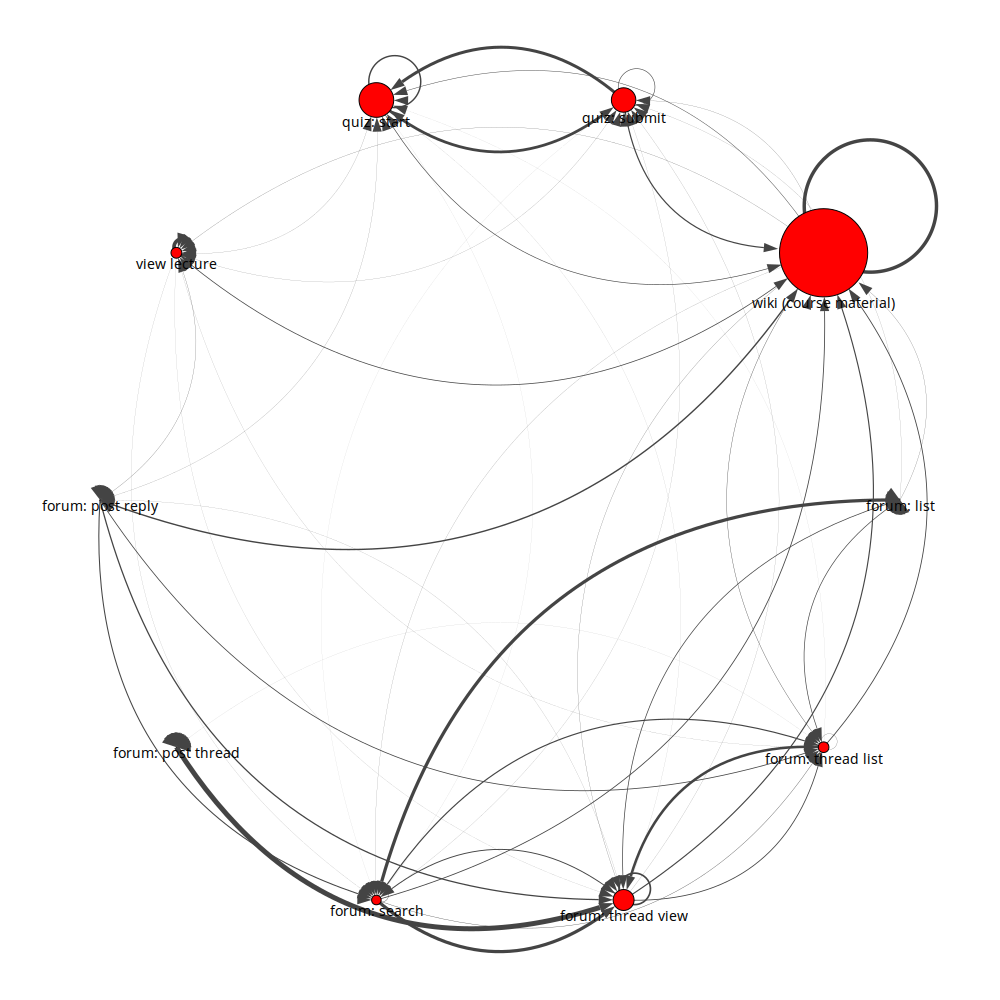
\includegraphics[width=\textwidth]{figures/text-6state/state0.png}
    \caption{An example ``quiz taking'' state.}
    \label{fig:practice-quiz-state}
  \end{subfigure}%
  \begin{subfigure}[t]{0.5\textwidth}
    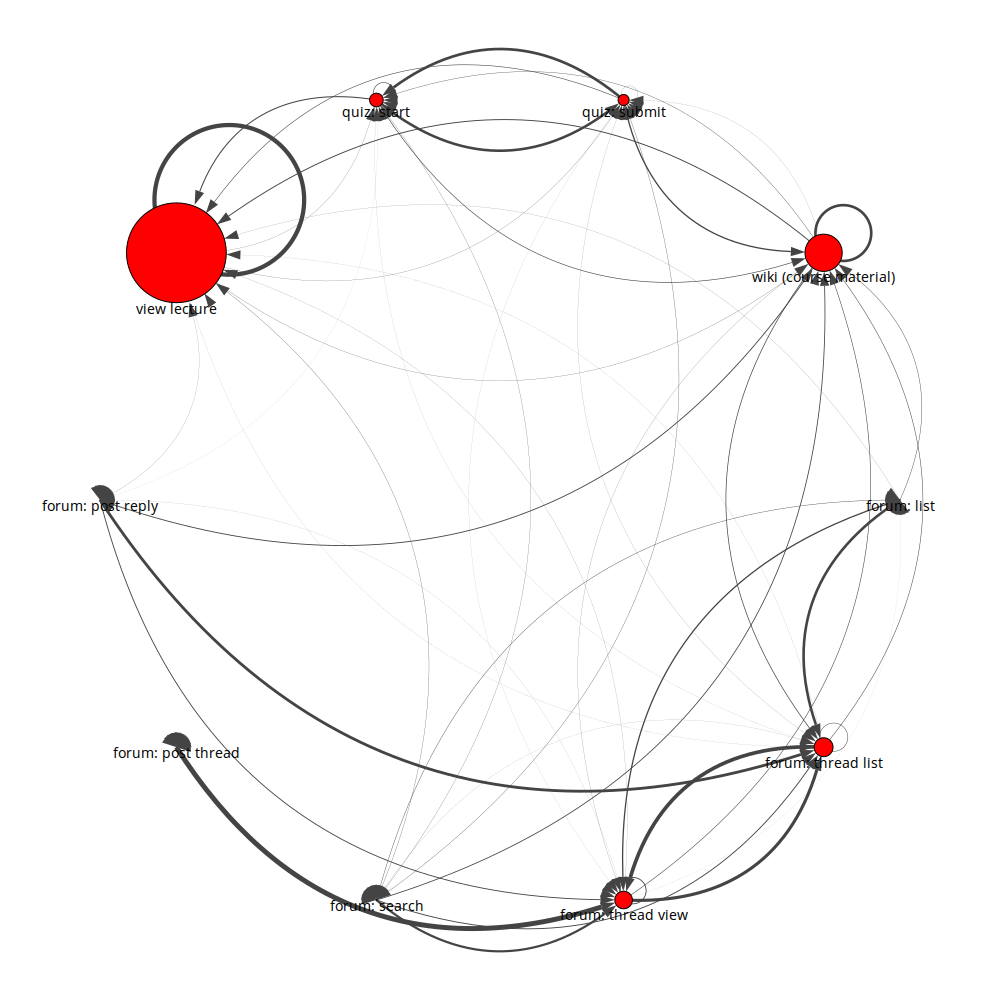
\includegraphics[width=\textwidth]{figures/text-6state/state1.png}
    \caption{An example ``lecture viewing'' state.}
    \label{fig:lecture-viewing-state}
  \end{subfigure}
  \caption{Two example states found by the 6-state TL-HMM.}
  \label{fig:states}
\end{figure*}

Figure~\ref{fig:states} includes two such representations we learned. The
first corresponds to a ``quiz taking'' state whereas the second corresponds
to a ``lecture viewing'' state. Clearly, our unsupervised method can
uncover states that do indeed correspond to student behavior modes that we
would expect to find a priori.

We also argue that it is important that the latent state representation be
a Markov model rather than just a discrete distribution over actions in
$\mathbf{A}$ (as would be the case for a traditional single-layer HMM). We
can observe why if we take a closer look at each of the two latent state
representations in Figure~\ref{fig:states} and look at their forum
component (bottom right). We can see that the relative probability of the
forum activities is roughly the same between these states, but the
\emph{transitions} are quite different. In
Figure~\ref{fig:practice-quiz-state} we have a relatively low probability
of walking from the ``forum thread view'' action back to the ``forum thread
list'' action, but in Figure~\ref{fig:lecture-viewing-state} we actually
observe a very strong link in this direction. This difference highlights an
important distinction between these two latent states: in the first you are
more likely to visit the forum \emph{looking for a particular post}, where
in the second you are more likely to visit the forum \emph{to browse
existing posts}. Thus, capturing the action transition matrix within a
latent state is important for capturing detailed insights involving bigrams
of actions.

% highlight interesting latent states discovered; make arguments that
% motivate why it's useful to have a Markov model as the latent state
% representation (capturing transitions between actions is useful and
% more meaningful than just using a discrete distribution as the latent
% state representation); show how the learned state representations differ
% between the two MOOCs

\subsection{Varying the Number of Latent States}
% show what happens as we vary k (particularly interesting to see 2 -> 3
% hidden state change, as the forum "topic" appears suddenly); argue that
% this allows the model to capture behavior patterns at different levels of
% granularity

\subsection{Transitions Between Latent States}
% using k=6, show that we can uncover interesting patterns in how students
% transition between the different latent states; argue that this discovery
% is interesting and unique to our formulation and could not be discovered
% before


\section{Conclusion}
% summarize the main contributions of the paper; summarize the experimental
% results; argue again for our novelty; discuss future directions
We proposed a two-layer hidden Markov model for MOOC student behavior
modeling in an unsupervised learning framework on large collections of
actions extracted from MOOC log data. This model is different from existing
methods in that it treats behavior patterns as a sequence of \emph{latent
states}, rather than assigning these states in a rule-based manner. It
captures the variable behaviors of students over time, and allows
analysis at different levels of granularity.

We showed that such a model does in fact capture meaningful behavior
patterns and produces descriptions of these behavior patterns that are easy
to interpret. We argued that it is important to capture student behavior
patterns with more sophisticated models than simple discrete distributions
over actions in order to capture information present in bigrams of actions
(or above). By varying the number of latent
states inferred, we showed that the model is flexible and can capture
patterns of differing levels of specificity in this way.  Finally, we
investigated whether we can detect differences in student behavior patterns
as they correlate with course performance. Specifically, we demonstrated
that high-performing students produce substantially different HMM
transition diagrams that tend to show longer concentration span in quiz-taking
and more active  forum participation as compared with the average students.

\subsection{Future Work}

Although we only experimented with our model on two MOOCs, the model is
completely general and can be easily applied to analyze the log of any
other course to enable deep understanding of student behaviors as well as
the correlations of such behaviors and other variables such as grades. We
plan to develop a MOOC log analysis system based on the proposed model to
both facilitate education research and help instructors improve course
design.

Our model can empower many new comparative analyses. For example, we could
now look at how behavior patterns change between different offerings of
the same MOOC to understand how changes in course structure or materials
influences student behavior. Individual students can now also be compared
against each other or against groups. For example, by decoding the latent
state sequences for each student, we can measure how ``surprising'' their
latent state transition sequence is relative to the average we would expect
according to the model, or to the average ``perfect'' student, etc. We can
now investigate how certain behavioral patterns correlate with properties
of a student (e.g., demographics, prior aptitude, etc.). After decoding the
students' latent state sequences, we could also correlate course-wide
drifts in these latent states with events in a course. For example, we
might be able to automatically discover difficult or confusing parts of a
course by noticing spikes in the distribution of students over latent
states over time.

Our model does not explicitly model drop-out like
\citet{Kizilcec:2013:LAK}, but doing so is an obvious extension. Our model
should be able to provide predictions of when a student is ``at risk'' for
dropping out under such an extension.

Currently, the model learns a transition matrix over the latent states that
is \emph{shared} across all students. It would be interesting to instead
learn a different latent state transition matrix for each individual
student, but keep the second-level Markov models shared. This would provide
the model with more flexibility which may be desirable itself, but would
also naturally result in a description of a student (via his or her HMM
transitions) that could be incorporated into existing supervised learning
techniques that try to predict student outcomes for understanding
which of the latent behavior patterns discovered by 2L-HMM are most predictive
of the performance of student learning.

There is more recent work on better learning algorithms for mixtures of
Markov models~\citep{Gupta:2016:NIPS}. It would be worth exploring whether
the advances proposed in this and similar work can be applied to our model
to address some of the concerns surrounding our use of the EM algorithm for
our parameter estimation.


\section{Acknowledgments}
\preprintonly{\acknowledgments{}}
\finalonly{\acknowledgments{}}
\submissiononly{(Anonymized for blind reviewing.)}
\bibliography{bib}
\end{document}
